\documentclass[tikz,border=8pt]{standalone}
\usepackage{amsmath}
\usepackage{pgfplots}
\pgfplotsset{compat=1.18}

\definecolor{ink}{HTML}{21352F}
\definecolor{teal}{HTML}{087F7B}
\definecolor{blue}{HTML}{4B77A8}
\definecolor{gold}{HTML}{C58B2A}
\definecolor{rose}{HTML}{B65A62}

\begin{document}
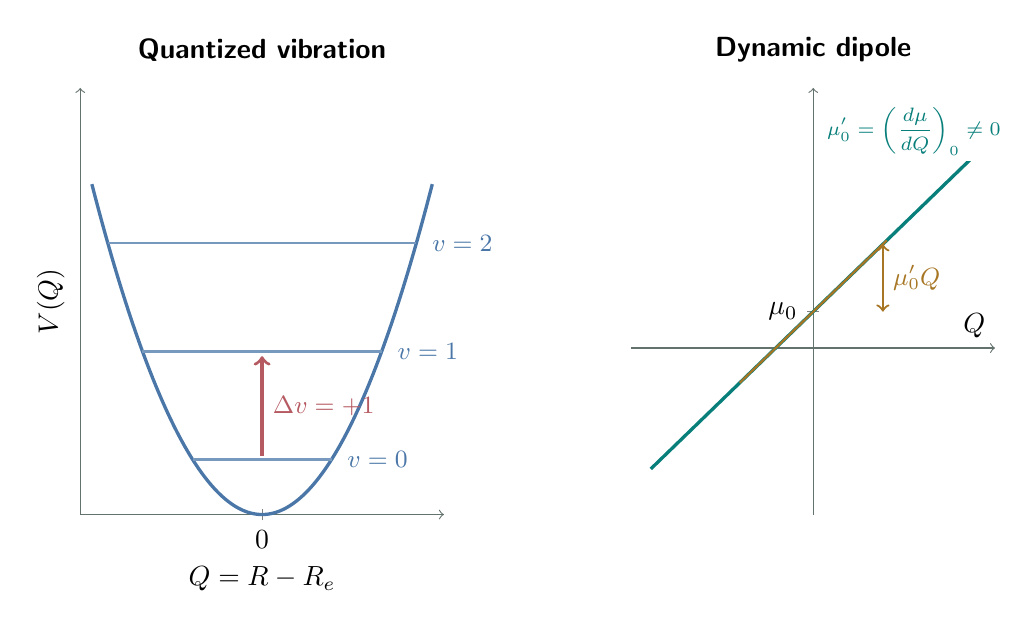
\begin{tikzpicture}[font=\sffamily]
  \begin{axis}[
    at={(0cm,0cm)},anchor=south west,
    width=6.2cm,height=7.0cm,
    xmin=-2.35,xmax=2.35,ymin=0,ymax=4.5,
    axis lines=left,
    axis line style={draw=ink!70,->},
    xlabel={$Q=R-R_e$},ylabel={$V(Q)$},
    xtick={0},ytick=\empty,
    title={\bfseries Quantized vibration},
    clip=false
  ]
    \addplot[blue,very thick,domain=-2.2:2.2,samples=140]
      {.72*x^2};
    \foreach \lev/\lab in {.58/0,1.72/1,2.86/2}{
      \pgfmathsetmacro{\dx}{sqrt(\lev/.72)}
      \pgfmathsetmacro{\xn}{\dx+.08}
      \edef\levelcommand{
        \noexpand\draw[blue!75,thick]
          (axis cs:-\dx,\lev)--(axis cs:\dx,\lev);
        \noexpand\node[blue,font=\noexpand\small,anchor=west]
          at (axis cs:\xn,\lev) {$v=\lab$};
      }
      \levelcommand
    }
    \draw[rose,very thick,->]
      (axis cs:0,.62)--(axis cs:0,1.67)
      node[midway,right,font=\small] {$\Delta v=+1$};
  \end{axis}

  \begin{axis}[
    at={(7.0cm,0cm)},anchor=south west,
    width=6.2cm,height=7.0cm,
    xmin=-2.35,xmax=2.35,ymin=-1.6,ymax=2.5,
    axis lines=middle,
    axis line style={draw=ink!70,->},
    xlabel={$Q$},ylabel={},
    xtick={0},ytick={.35},
    yticklabels={$\mu_0$},
    title={\bfseries Dynamic dipole},
    clip=false
  ]
    \addplot[teal,very thick,domain=-2.1:2.1,samples=3]
      {.35+.72*x};
    \draw[gold!85!black,thick]
      (axis cs:-.95,-.334)--(axis cs:.95,1.034);
    \draw[gold!85!black,thick,<->]
      (axis cs:.9,.35)--(axis cs:.9,.998)
      node[midway,right,font=\small] {$\mu_0'Q$};
    \node[teal,font=\scriptsize,align=center,fill=white,inner sep=2pt]
      at (axis cs:1.30,2.08)
      {$\displaystyle\mu_0'=
      \left(\frac{d\mu}{dQ}\right)_0\ne0$};
  \end{axis}
\end{tikzpicture}
\end{document}
